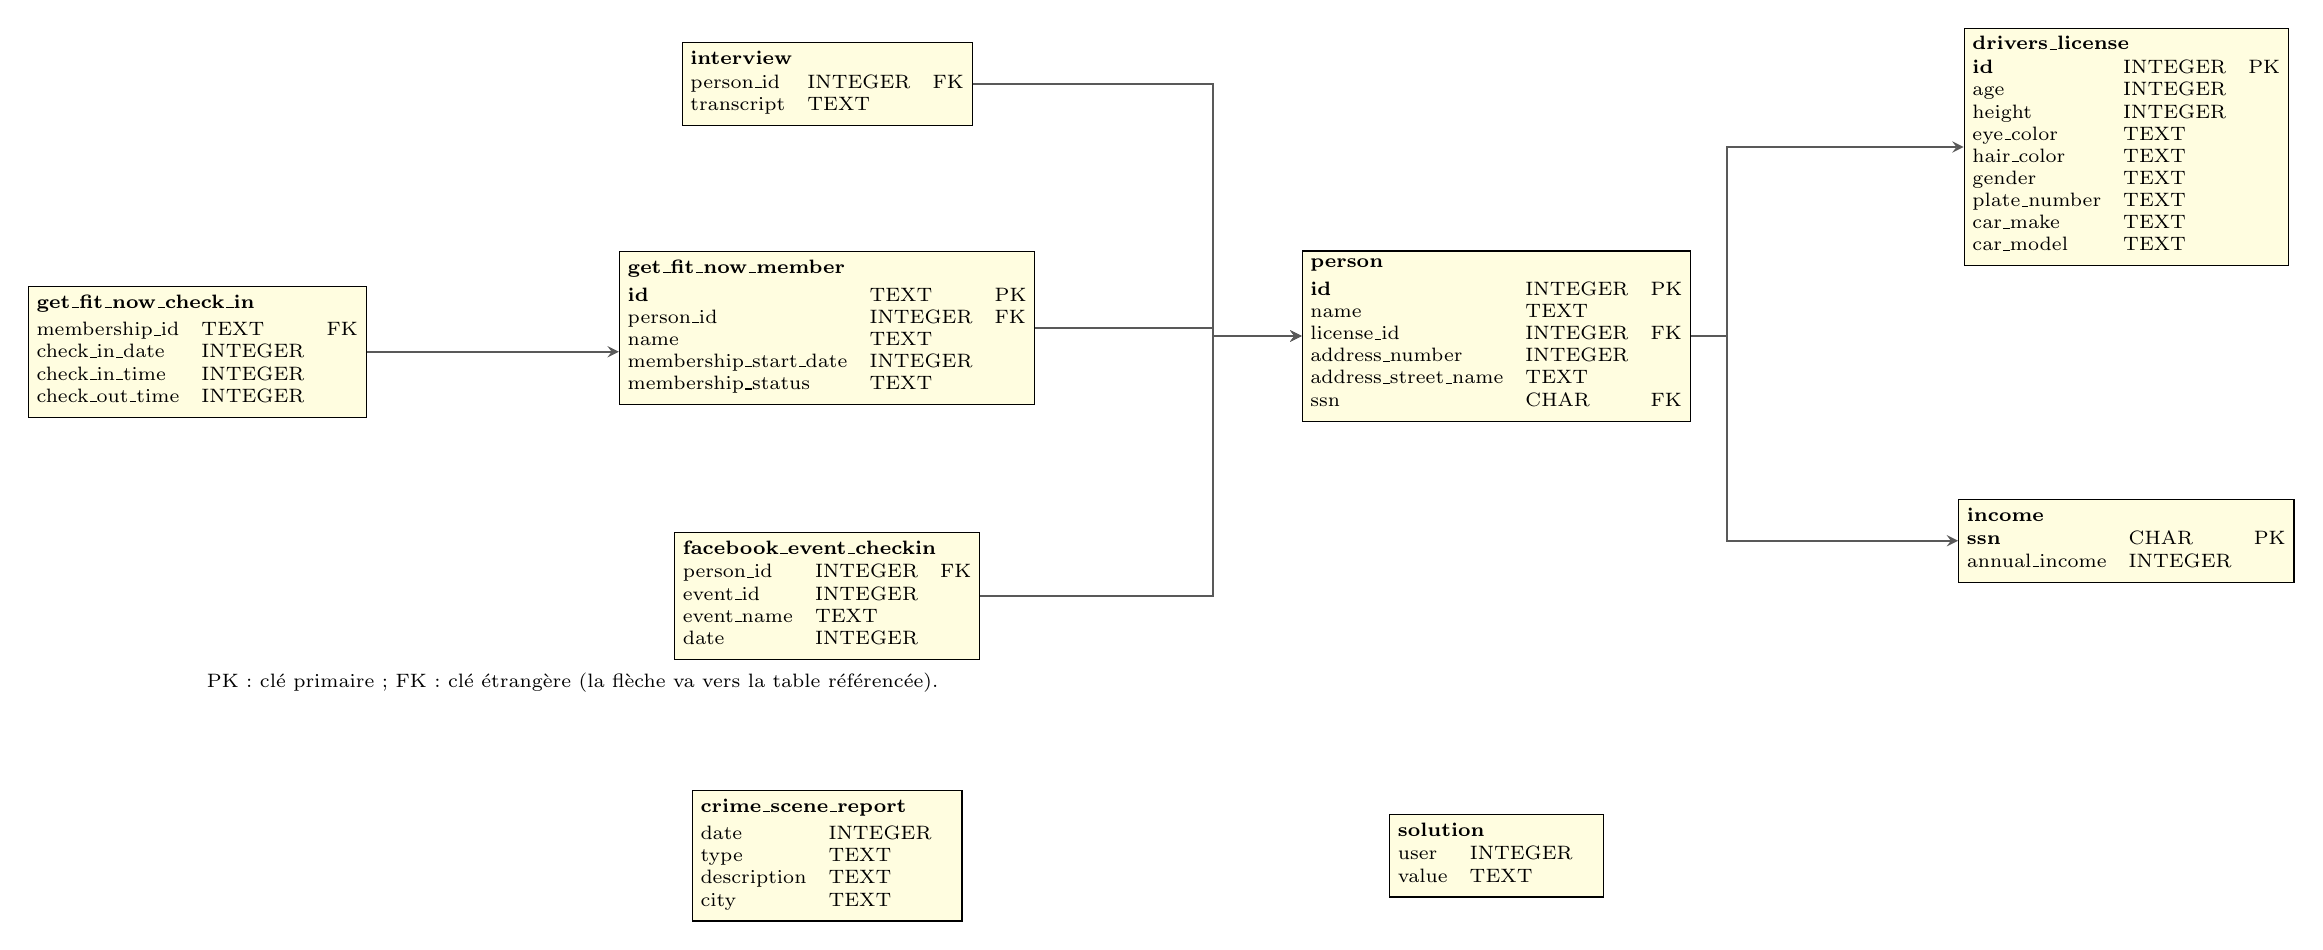
\begin{tikzpicture}[x=1cm,y=1cm,tbl/.style={draw,fill=yellow!12,inner sep=3pt,font=\scriptsize,align=left},fk/.style={->,>=stealth,thick,gray!70!black}]
\node[tbl] (get_fit_now_check_in) at (0.0,0.0) {\textbf{get\_fit\_now\_check\_in}\\[2pt]\begin{tabular}{@{}l@{\quad}l@{\quad}l@{}}
membership\_id & TEXT & FK\\
check\_in\_date & INTEGER & \\
check\_in\_time & INTEGER & \\
check\_out\_time & INTEGER & \\
\end{tabular}};
\node[tbl] (interview) at (8.0,3.4) {\textbf{interview}\\[2pt]\begin{tabular}{@{}l@{\quad}l@{\quad}l@{}}
person\_id & INTEGER & FK\\
transcript & TEXT & \\
\end{tabular}};
\node[tbl] (get_fit_now_member) at (8.0,0.3) {\textbf{get\_fit\_now\_member}\\[2pt]\begin{tabular}{@{}l@{\quad}l@{\quad}l@{}}
\textbf{id} & TEXT & PK\\
person\_id & INTEGER & FK\\
name & TEXT & \\
membership\_start\_date & INTEGER & \\
membership\_status & TEXT & \\
\end{tabular}};
\node[tbl] (facebook_event_checkin) at (8.0,-3.1) {\textbf{facebook\_event\_checkin}\\[2pt]\begin{tabular}{@{}l@{\quad}l@{\quad}l@{}}
person\_id & INTEGER & FK\\
event\_id & INTEGER & \\
event\_name & TEXT & \\
date & INTEGER & \\
\end{tabular}};
\node[tbl] (person) at (16.5,0.2) {\textbf{person}\\[2pt]\begin{tabular}{@{}l@{\quad}l@{\quad}l@{}}
\textbf{id} & INTEGER & PK\\
name & TEXT & \\
license\_id & INTEGER & FK\\
address\_number & INTEGER & \\
address\_street\_name & TEXT & \\
ssn & CHAR & FK\\
\end{tabular}};
\node[tbl] (drivers_license) at (24.5,2.6) {\textbf{drivers\_license}\\[2pt]\begin{tabular}{@{}l@{\quad}l@{\quad}l@{}}
\textbf{id} & INTEGER & PK\\
age & INTEGER & \\
height & INTEGER & \\
eye\_color & TEXT & \\
hair\_color & TEXT & \\
gender & TEXT & \\
plate\_number & TEXT & \\
car\_make & TEXT & \\
car\_model & TEXT & \\
\end{tabular}};
\node[tbl] (income) at (24.5,-2.4) {\textbf{income}\\[2pt]\begin{tabular}{@{}l@{\quad}l@{\quad}l@{}}
\textbf{ssn} & CHAR & PK\\
annual\_income & INTEGER & \\
\end{tabular}};
\node[tbl] (crime_scene_report) at (8.0,-6.4) {\textbf{crime\_scene\_report}\\[2pt]\begin{tabular}{@{}l@{\quad}l@{\quad}l@{}}
date & INTEGER & \\
type & TEXT & \\
description & TEXT & \\
city & TEXT & \\
\end{tabular}};
\node[tbl] (solution) at (16.5,-6.4) {\textbf{solution}\\[2pt]\begin{tabular}{@{}l@{\quad}l@{\quad}l@{}}
user & INTEGER & \\
value & TEXT & \\
\end{tabular}};
\draw[fk] (get_fit_now_check_in.east) -- (get_fit_now_member.west|-get_fit_now_check_in.east);
\draw[fk] (get_fit_now_member.east) -- (12.9,0 |- get_fit_now_member.east) |- (person.west);
\draw[fk] (interview.east) -- (12.9,0 |- interview.east) |- (person.west);
\draw[fk] (facebook_event_checkin.east) -- (12.9,0 |- facebook_event_checkin.east) |- (person.west);
\draw[fk] (person.east) -- ++(0.45,0) |- (drivers_license.west);
\draw[fk] (person.east) -- ++(0.45,0) |- (income.west);
\node[font=\scriptsize,anchor=west] at (0,-4.2) {PK : clé primaire ; FK : clé étrangère (la flèche va vers la table référencée).};
\end{tikzpicture}